% Chapter 1

\chapter{Introduction} % Main chapter title

\label{Chapter1} % For referencing the chapter elsewhere, use \ref{Chapter1} 

%----------------------------------------------------------------------------------------

First of all is important to understand at least generically what is the AEgIS experiment at the CERN and what are its goals. The acronym AEgIS stands for "Antimatter Experiment: gravity, Interferometry, Spectroscopy", this experiment aims to measure weak equivalence principle for antimatter. In the first part of this chapter are explained some particulars about this experiment, in the second part is introduced gAn Web, the main topic of this document, the application that allows the physicists to do data analysis in the AEgIS experiment environment easily, by a web interface. 

\section{AEgIS experiment}


\begin{figure}[H]
\centering
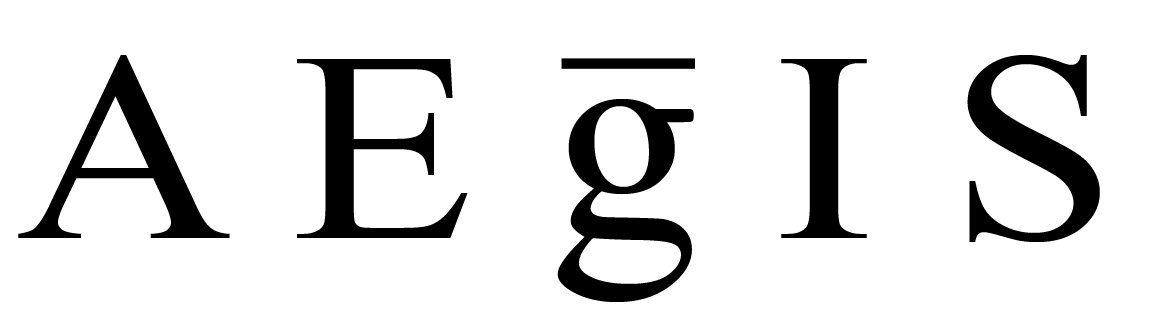
\includegraphics[scale=0.25]{aegisLogo.png} 
\caption{AEgIS's Logo}
\end{figure}

The weak equivalence principle, also known as universality of free fall, states that in the same field all bodies fall with the same acceleration, regardless of the mass and the composition. This principle has been thoroughly tested for the matter, but not for the antimatter: the most important goal of AEgIS experiment is to measure the weak equivalence principle for the anti-matter; to test this principle AEgIS measures gravitational interaction between matter (the earth) and anti-matter (anti-hydrogen). In the context of neutral antimatter, the gravitational interaction is of high interest, because it can potentially revealing new forces that violate the weak equivalence principle. Thomas Phillips, from Duke University, says: "If antimatter fell down faster, it would mean the discovery of at least one new force, probably two. If it fell up, it would mean our understanding of general relativity is incorrect". In a practical point of view AEgIS tries to mesure the time of flight and the vertical displacement of anti-hydrogen, by a moire deflectometer: this process is quite complex, and it is easier explain it by the following two images [TODO INSERT-THE-NUMBER-OF-THE-IMAGE].

\begin{figure}[H]
\centering
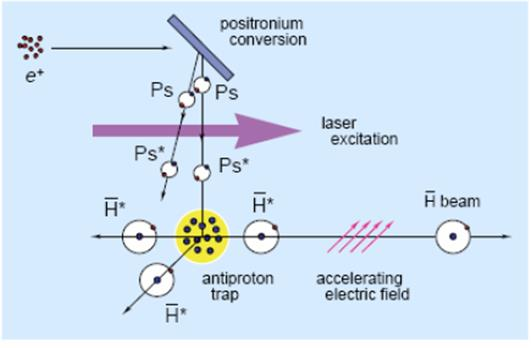
\includegraphics[scale=0.5]{AEgISScheme.png} 
\caption{AEgIS's Scheme, taken from "AEgIS experiment at CERN: measuring antihydrogen free-fall in Earth’s gravitational field to test WEP with antimatter" TODO INSERT-bibliographical-reference}
\end{figure}

In this first image we can see the process that allows to create some anti-hydrogen. To correctly explain this process it is better start with some definitions:


\begin{enumerate}

% 1
\item Positron: it is the correspondent of the electron in the anti-matter. It is an anti-electron, so an electron with positive electrical charge. It is indicated by "e+".

% 2
\item Positronium: it is an unstable system consisting of an electron and a positron, bound together into an exotic atom. It is indicated with $ {Ps} $.

% 3
\item Antiporoton: it is the antiparticle of the proton. Antiprotons are stable, but they are typically short-lived since any collision with a proton will cause both particles to be annihilated in a burst of energy. It is indicated with $ \overline{p} $ (pronunced P-Bar).

% 4
\item Antihydrogen: it is the antimatter counterpart of hydrogen. Whereas the common hydrogen atom is composed of an electron and proton, the antihydrogen atom is made up of a positron and antiproton. It is indicated with $ \overline{H} $ (pronunced H-Bar).


% 5
\item Antiproton trap: a devices that uses an axial magnetic field to transversely confine charged particles, in this case antiprotons.


\end{enumerate}

The process shown in the image is the following: a beam of positrons (that comes from a 22Na radioactive source) is accelerated and driven to collide against a "positron-positronium converter" (that is a mesoporous silica film). This process creates positronium, that needs to be excited by lasers, to reach the Rydberg State. The positronium in Rydberg state is indicated by $ {Ps*} $, it has a longer life than the unexcited positronium, and can be driven to fly into an antiproton trap.

Antiprotons are provided in this way:
Protons collide with nuclei inside a metal cylinder called "target". About four proton-antiproton pairs are produced in every million collisions, and is possible to separate antiprotons from matter using magnetic fields. The following step is to guide antiprotons toward the AD (Antiproton Decelerator) where they are slowed down (it is easier work with slow antiprotons). To carry out AEgIS experiment antiproton must be trapped and conserved inside an antiproton trap, where magnetic fields force the charged antiparticles to spiral around the magnetic field lines, and electric fields confine them along the magnetic axis.

In the following step $ {Ps*} $ and $ \overline{p} $ can combine themselves to generate excited antihydrogen ($ \overline{H}* $) and electrons. The antihydrogen beam is accelerated using an electric field towards a Moiré deflectometer, during the travel it decays to ground state.  


\begin{figure}[H]
\centering
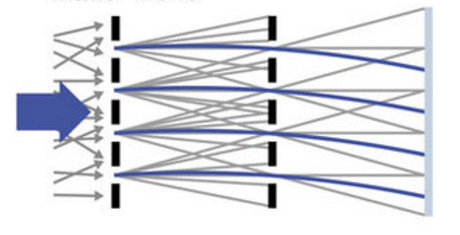
\includegraphics[scale=0.5]{MoireDeflectometer.png} 
\caption{Moiré Deflectometer's Scheme, taken from "A
http://www.nature.com/articles/ncomms5538" TODO INSERT-bibliographical-reference}
\end{figure}

In the second image is visible how does the Moirè deflectometer work.
A antihydrogen beam is thrown toward two subsequent gratings that restrict the transmitted particles to well-defined trajectories. The trajectories are inflected by a force (in this case the force related to $ {m*g} $) and follows a parabolic path. At the final part of the deflectometer there is a detector that shows where the antimatter annihilates, so is possible to compare the expected trajectories without forces with the obtained trajectories, and measure the force.


\begin{figure}[H]
\centering
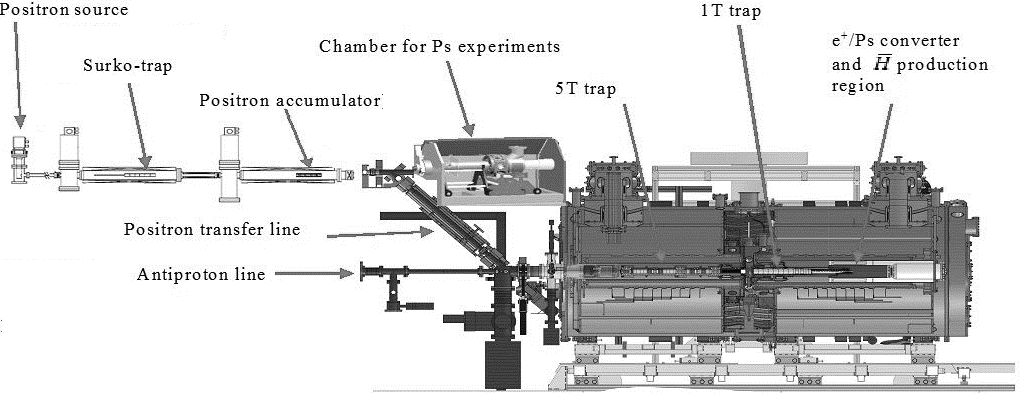
\includegraphics[scale=0.5]{SchemeMachineSetUp.png} 
\caption{AEgIS apparatus set up, taken from "AEgIS experiment at CERN: measuring antihydrogen free-fall in Earth’s gravitational field to test WEP with antimatter" TODO INSERT-bibliographical-reference}
\end{figure}

\section{User friendly Data analysis: gAn Web}

GAn Web is a web application, that creates a user friendly web interface, based on the most important human-machine interaction principles, between the users and a pre-existing data analysis application named gAn.
This document's most important goal is explain in detail how gAn Web works, how and why it was created, what are the reasons for the choices made. 

GAn Web is based on the pre-existent stand-alone program gAn, that allows users to do data analysis using a Linux terminal as interface. In turn, gAn is based on Root Data Analysis Framework, a vast and modular scientific software framework that provides all the functionalities needed to deal with big data processing, statistical analysis, visualisation and storage of physical data. GAn exploits and organizes the functionalities of Root, the resulting software is practical and achieves his goals, but a web interface can improve it in two ways:

\begin{enumerate}

% 1
\item gAn is a stand-alone program based on Root, installable on the user's machine; the user has to install the correct version of Root to avoid compatibility problems (Root is still not perfectly version independent: different versions can lead to different behaviours). Furthermore, this kind of program is continuously changing, the performed analysis is continuously improved, so the installed version of gAn is not final and unchangeable, and the user musts often update it. Instead, a centralized version installed on a server, with services accessible from a normal browser by the user can avoid (at least reduce) this kind of problems and be more usable.    
 

% 2
\item a Linux terminal interface is practical for expert users, but a web based interface can be more attractive for new users, and, if well done, can be easier to use. It is important to notice that the users are physicists, not necessarily specialized in computer science, so, create a friendly and easily learnable interface can avoid them problems and time wasting.   


\end{enumerate}


The goal of gAn Web is to allow users to do analysis through a more friendly web interface, without install nothing on their machine. In the following image there is a schema that shows how this program is organized.

\begin{figure}[H]
\centering
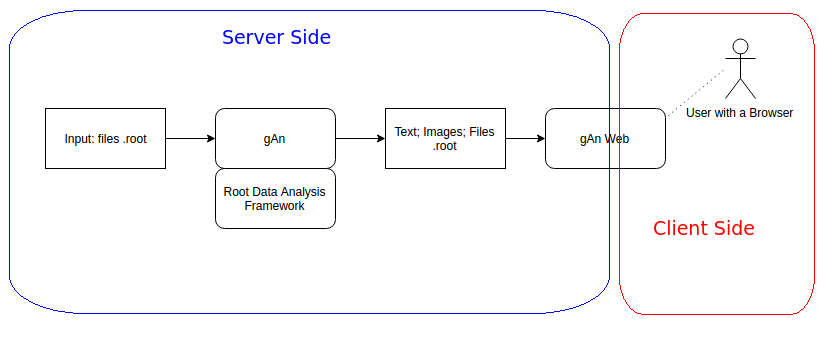
\includegraphics[scale=0.5]{GeneralGAnSchema.png} 
\caption{gAn - gAn Web simple scheme}
\end{figure}

The input of this system is represented by a set of files .root. These are raw, very big, binary files, incomprehensible to humans, generated by the hardware (mostly by detectors) of the AEgIS experiment, they need the Root Data Analysis Framework to be interpreted. These files contain a lot of information, too much and too disorganized to be helpful for the analysis. GAn can read these root files, make an ordered and organized analysis, extract the most important information, and produce an output that consists of a text with the most important informations, comments, and eventual error logs, a folder with some images, that can summarise effectively the most important points of the analysis, and some other .root files, with useful informations that allow gAn Web to make further processing. GAn Web can close the cycle acting as intermediary between the users and gAn: gAn Web can receive requests from the users, configure gAn to satisfy these requests, and deliver to the users exactly what they need.


